\section{Wstęp}
%\subsection{Geneza}
Tematem projektu, którego dotyczy ta praca jest: „Projekt i~realizacja stanowiska laboratoryjnego do badania zależności czasowych w~sieci EtherCAT". Zagadnienia związane z~tworzeniem oprogramowania dla sterowników przemysłowych są dla autora niezwykle interesujące, a zrealizowany projekt miał na~celu dalsze pogłębienie jego wiedzy z tego zakresu. Wyboru tego konkretnego tematu autor dokonał, ponieważ protokół EtherCAT jest jeszcze nowością i według wielu źródeł stanowi przyszłość branży informatyki przemysłowej \cite{art1_etherCAT, art2_etherCAT}, a~praca nad tym tematem wydaje się być pomocna i~wartościowa w przyszłej pracy zawodowej lub na~ewentualnym dalszym etapie kształcenia.

\subsection{Stanowisko laboratoryjne}
Na potrzeby realizacji projektu wykorzystano dwa różne istniejące stanowiska laboratoryjne, które składały się~z~elementów opisanych w Tabeli~\ref{stanowiska}.
\begin{table}[!htb]
\begin{center}
\begin{tabular}{| p{0.5\textwidth} | p{0.5\textwidth} |}\hline
Stanowisko typu CP (Rysunek~\ref{stanowisko:cp}) & Stanowisko typu CX (Rysunek~\ref{stanowisko:cx})  \\\hline
\begin{enumerate}[leftmargin=7mm]
\setlength{\itemsep}{5pt}
\setlength{\parskip}{0pt}
\setlength{\parsep}{0pt}
\item 2~silniki AM3021-0C00-0000,
\item Wyspa EK1100 z~zestawem modułów~IO:
\begin{itemize}[leftmargin=3mm]
\setlength{\itemsep}{3pt}
\setlength{\parskip}{0pt}
\setlength{\parsep}{0pt}
\item Terminal sieci EtherCAT EK1100,
\item 2-kanałowy moduł wyjść analogowych EL4132,
\item 4-kanałowy moduł wejść cyfrowych EL1004,
\item 2 4-kanałowe moduły wyjść cyfrowych EL2004,
\item 2-kanałowy moduł wejść analogowych EL3102,
\end{itemize}
\item Napęd serwomechnizmów AX5203 (2~osiowy),
\item Komputer przemysłowy C6925,
\item Zasilacz.
\end{enumerate}
&
\begin{enumerate}[leftmargin=7mm]
\setlength{\itemsep}{5pt}
\setlength{\parskip}{0pt}
\setlength{\parsep}{0pt}
\item 2~silniki AM3021-0C00-0000,
\item Zestaw modułów IO:
\begin{itemize}[leftmargin=3mm]
\setlength{\itemsep}{3pt}
\setlength{\parskip}{0pt}
\setlength{\parsep}{0pt}
\item 2-kanałowy moduł wyjść analogowych EL4132,
\item 4-kanałowy moduł wejść cyfrowych EL1004,
\item 2 4-kanałowe moduły wyjść cyfrowych EL2004,
\item 2-kanałowy moduł wejść analogowych EL3102,
\end{itemize}
\item Terminal sieci EtherCAT EK1100,
\item Napęd serwomechnizmów AX5203 (2~osiowy),
\item Modułowy komputer przemysłowy CX1020:
\begin{itemize}[leftmargin=3mm]
\setlength{\itemsep}{3pt}
\setlength{\parskip}{0pt}
\setlength{\parsep}{0pt}
\item Interfejs USB/DVI CX1020-N010 ,
\item Ethernet CX1020-N000,
\item CPU CX1020-0113,
\item Zasilacz CPU i magistrali I/O CX1100,
\end{itemize}
\item Zasilacz.
\end{enumerate}
\\\hline                                            
\end{tabular}
\end{center}
\vspace*{-6mm}
  \caption{Dostępne stanowiska laboratoryjne}
	\label{stanowiska}
\end{table}

\begin{figure}[htbp]
 \centering
        \tikzstyle{background grid}=[draw, black!50,step=.25cm]
	\begin{tikzpicture}[node distance=1cm, auto]%, show background grid]
	\tikzset{
    	mynode/.style={rectangle,rounded corners,draw=black, top color=white, bottom color=yellow!50,very thick, inner sep=1em, minimum size=3em, 		text centered, text width=3cm},
    	mynodemini/.style={rectangle,rounded corners,draw=black, top color=white, bottom color=yellow!50,very thick, inner sep=.5em, text centered},    	
	    myarrow/.style={->, >=latex', shorten >=1pt, thick},
	    myline/.style={-, =latex', shorten >=1pt, rounded corners, ultra thick},
	    mylabel/.style={text width=7em, text centered} 
	} 
	\node[mynode] (plc) {Komputer \\ przemysłowy C6925};  
	\node [left=of plc] (laptop) {
\includegraphics[width=3cm]{images/laptop}};
	\node[mynode, right=of plc] (zasilacz) {Zasilacz};
	\node[below=2cm of plc] (dummy) {}; 
	\node[mynode, left=of dummy] (io) {Wyspa EK1100 z~zestawem modułów IO};  	 	 	
 	\node[mynodemini, left=of io] (io2) {EL1004};
 	\node[mynodemini, above=2mm of io2] (io1) {EL4132};  	
 	\node[mynodemini, above=2mm of io1] (io0) {EK1100};
 	\node[mynodemini, below=2mm of io2] (io3) {EL2004}; 	 	
 	\node[mynodemini, below=2mm of io3] (io4) {EL2004};
 	\node[mynodemini, below=2mm of io4] (io5) {EL3102};
 	\node [fit=(io0) (io1) (io2) (io3) (io4) (io5)] (fit) {};  
 	%\draw [decorate, xshift=-20pt,line width=4pt] (fit.south east) -- (fit.north east);
	\draw [decorate,decoration={brace, mirror,amplitude=10pt}, line width=1pt] (fit.south east) -- (fit.north east);
	
	\node[mynode, right=of dummy] (naped) {Napęd \\ serwomechnizmów AX5203};
	\node[below=2cm of naped] (dummy2) {}; 
	\node[mynode, left=of dummy2, text width=4cm](silnik1){Silnik \\ AM3021-0C00-0000};
	\node[mynode, right=of dummy2, text width=4cm](silnik2){Silnik \\ AM3021-0C00-0000};
	
	\draw[myline,black,dotted] (fit.east) ++(0.4, 0) -- (io.west);
	\draw[myline,blue] (laptop.east) -- ++(-1, 0) -- (plc.west);
	
	\draw[myline,black] (zasilacz.west) -- (plc.east);
	\draw[myline,black] (zasilacz.south) -- (io.north);
	\draw[myline,black] (zasilacz.south) -- (naped.north);	
	
	\draw[myline,purple] (io0.south) -- (io1.north);	
	\draw[myline,purple] (io1.south) -- (io2.north);
	\draw[myline,purple] (io2.south) -- (io3.north);		
	\draw[myline,purple] (io3.south) -- (io4.north);
	\draw[myline,purple] (io4.south) -- (io5.north);
	
	\draw[myline,yellow] (plc.south) -- (naped.north);	
	\draw[myline,yellow] (io.east) -- (naped.west);	

	\draw[myline, green, bend right=10] (naped.south) to (silnik1.north);
	\draw[myline, orange, bend left=10] (naped.south) to (silnik1.north);	
	\draw[myline, green, bend right=10] (naped.south) to (silnik2.north);
	\draw[myline, orange, bend left=10] (naped.south) to (silnik2.north);	
	%\draw[<->, >=latex', shorten >=2pt, shorten <=2pt, bend right=45, thick, dashed] 
    %(io.south) to node[auto, swap] {Competition}(naped.south); 
    
    \draw [purple, line width=6] (6,-1) -- (6.5,-1); \node[text width=2cm] at (7.65,-1.3) {EtherCAT (E-bus)};    
    \draw [yellow, line width=6] (6,-2) -- (6.5,-2); \node[text width=2cm] at (7.65,-2.3) {EtherCAT (skrętka)};
    \draw [blue, line width=6] (6,-3) -- (6.5,-3); \node at (7.5,-3) {Ethernet};
    \draw [black, line width=6] (6,-3.5) -- (6.5,-3.5); \node at (7.5,-3.5) {Zasilanie};
    \draw [green, line width=6] (6,-4) -- (6.25,-4); \draw [orange, line width=6] (6.25,-4) -- (6.5,-4); 
    \node [text width=2cm] at (7.75,-4.25) {Sterowanie silnikiem};    
\end{tikzpicture} 
\caption{Schemat stanowiska typu CP}
\label{stanowisko:cp}
\end{figure} %
\begin{figure}[htbp]
 \centering
        \tikzstyle{background grid}=[draw, black!50,step=.5cm]
	\begin{tikzpicture}[node distance=1cm, auto]%, show background grid]
	\tikzset{
    	mynode/.style={rectangle,rounded corners,draw=black, top color=white, bottom color=yellow!50,very thick, inner sep=1em, minimum size=3em, 		text centered, text width=3cm},
    	mynodemini/.style={rectangle,rounded corners,draw=black, top color=white, bottom color=yellow!50,very thick, inner sep=.5em, text centered},
	    myarrow/.style={->, >=latex', shorten >=1pt, thick},
	    myline/.style={-, =latex', shorten >=1pt, rounded corners, ultra thick},
	    mylabel/.style={text width=7em, text centered} 
	} 
	\node[mynode] (plc) {Modułowy komputer przemysłowy CX1020};  
	\node[mynode, above=of plc] (plc1) {CX1020-N010 \\ DVI/USB};
	\node[mynode, left=of plc1] (plc2) {CX1020-N000 \\ LAN};
	\node[mynode, right=of plc1] (plc3) {CX1020-0113 \\ CPU};
 	\node [fit=(plc1) (plc2) (plc3)] (fit) {}; 
 	\draw [decorate,decoration={brace,amplitude=10pt}, line width=1pt] (fit.south east) -- (fit.south west);
 		
	\node [left=of plc] (laptop) {
\includegraphics[width=3cm]{images/laptop}};
	\node[below=2cm of plc] (dummy) {}; 
	\node[mynode, left=of dummy] (io) {Zestaw  \\modułów~IO}; 
 	\node[mynodemini, left=of io] (io2) {EL1004};
	\node[mynodemini, above=2mm of io2] (io1) {EL4132};  	
 	\node[mynodemini, above=2mm of io1] (io0) {CX1100}; 	 	
 	\node[mynodemini, below=2mm of io2] (io3) {EL2004}; 	 	
 	\node[mynodemini, below=2mm of io3] (io4) {EL2004};
 	\node[mynodemini, below=2mm of io4] (io5) {EL3102};
 	\node [fit=(io0) (io1) (io2) (io3) (io4) (io5)] (fit2) {};  
 	%\draw [decorate, xshift=-20pt,line width=4pt] (fit.south east) -- (fit.north east);
	\draw [decorate,decoration={brace, mirror,amplitude=10pt}, line width=1pt] (fit2.south east) -- (fit2.north east);
 	 	 	 	 	 	
	\node[mynode, below=5mm of io, text width=1.6cm] (ek) {Terminal EK1100};  
	
	\node[mynode, right=of dummy] (naped) {Napęd \\ serwomechnizmów AX5203};
	\node[below=2cm of naped] (dummy2) {}; 
	\node[mynodemini, left=2mm of dummy2, text width=4cm](silnik1){Silnik \\ AM3021-0C00-0000};
	\node[mynodemini, right=2mm of dummy2, text width=4cm](silnik2){Silnik \\ AM3021-0C00-0000};

	\draw[myline,black,dotted] (fit.south) ++(0, -0.4) -- (plc.north);	
	\draw[myline,black,dotted] (fit2.east) ++(0.4, 0) -- (io.west);
	\draw[myline,blue] (laptop.east) -- ++(-1, 0) -- (plc.west);
	
	\draw[myline,purple] (plc.south) -- (io.north);	
	\draw[myline,purple] (io.south) -- (ek.north);
	\draw[myline,purple] (io0.south) -- (io1.north);	
	\draw[myline,purple] (io1.south) -- (io2.north);
	\draw[myline,purple] (io2.south) -- (io3.north);		
	\draw[myline,purple] (io3.south) -- (io4.north);
	\draw[myline,purple] (io4.south) -- (io5.north);
				
	\draw[myline,yellow] (ek.east) -- (naped.west);	

	\draw[myline, green, bend right=10] (naped.south) to (silnik1.north);
	\draw[myline, orange, bend left=10] (naped.south) to (silnik1.north);	
	\draw[myline, green, bend right=10] (naped.south) to (silnik2.north);
	\draw[myline, orange, bend left=10] (naped.south) to (silnik2.north);	
	%\draw[<->, >=latex', shorten >=2pt, shorten <=2pt, bend right=45, thick, dashed] 
    %(io.south) to node[auto, swap] {Competition}(naped.south); 
    
    \draw [purple, line width=6] (6,-1) -- (6.5,-1); \node[text width=2cm] at (7.65,-1.3) {EtherCAT (E-bus)};    
    \draw [yellow, line width=6] (6,-2) -- (6.5,-2); \node[text width=2cm] at (7.65,-2.3) {EtherCAT (skrętka)};
    \draw [blue, line width=6] (6,-3) -- (6.5,-3); \node at (7.5,-3) {Ethernet};
    \draw [black, line width=6] (6,-3.5) -- (6.5,-3.5); \node at (7.5,-3.5) {Zasilanie};
    \draw [green, line width=6] (6,-4) -- (6.25,-4); \draw [orange, line width=6] (6.25,-4) -- (6.5,-4); 
    \node [text width=2cm] at (7.75,-4.25) {Sterowanie silnikiem};    
\end{tikzpicture} 
\caption{Schemat stanowiska typu CX.}
\label{stanowisko:cx}
\end{figure}
 %

\subsubsection{Sterownik PLC}
W~realizacji wykorzystane zostały stanowiska firmy Beckhoff wyposażone w jednostki centralne pracujące pod kontrolą Windowsa CE (Microsoft Windows Compact Edition). Na~jednostce takiej uruchamiane są programy do~sterowania z poziomu komputera (ang. Soft PLC). Jest to rozwiązanie alternatywne dla~klasyczny sterowników swobodnie programowalnych w~postaci dedykowanego urządzenia (ang.~Hard~PLC), nazywanych przez niektórych prawdziwymi (ang.~True~PLC).
Koncepcja~ta powstała i~jest rozwijana, ponieważ te~klasyczne sterowniki posiadają zbyt małe możliwości obliczeniowe oraz szybkość działania jednostki centralnej. W~tradycyjnych rozwiązaniach niestety zwiększanie tych możliwości (ilość dostępnej pamięci oraz szybkości działania) powoduje bardzo szybki wzrost ceny gotowego urządzenia.
Niezbędnym elementem konfiguracji zestawu, który przekształcamy w~,,soft PLC'' jest karta komunikacyjna umożliwiająca połączenie sterownika z~modułami sygnałowymi i~wykonawczymi na~obiekcie z~wykorzystaniem sieci przemysłowej.
Przykładowe zastosowanie programu do~sterowania z~poziomu komputera zostało szczegółowo opisane w \cite{art_softPLC}.
Tego typu podejście i~rozwiązanie~ma następujące zalety:
\begin{itemize}
\item duże zwiększenie możliwości obliczeniowych przy stosunkowo niewielkim wzroście kosztów,
\item możliwość integracji PLC i~systemu SCADA na~jednym urządzeniu (podobnie jak w~panelach operatorskich ze~zintegrowanymi sterownikami~PLC),
\item możliwość zastosowania istniejącej infrastruktury na~obiekcie w~przypadku przebudowy, należy jedynie podmienić istniejący sterownik typu ,,hard'' na~jednostkę wyposażoną w~odpowiedni moduł komunikacyjny,
\item teoretycznie możliwość zastosowania istniejącego oprogramowania z jednostki ,,hard PLC'', po modyfikacji ewentualnych różnic między systemami.
\end{itemize}

Taki ,,sterownik PLC w komputerze PC'' wykorzystuje standardowe języki programowania sterowników~PLC (zgodność z~normą IEC~61131-3) do~tworzenia logiki sterującej takiej jak:
\begin{itemize}
\item IL -- \textbf{I}nstruction \textbf{L}ist to~tekstowy język programowania składający się z~serii instrukcji, z~których każda zaczyna~się z~nowej linii i~zawiera operator z~jednym lub więcej argumentem (zależnie od~funkcji),

\item LD -- \textbf{L}adder \textbf{D}iagram jest graficznym językiem programowania, który swoją struktura przypomina obwód elektryczny. Doskonały do~łączenia POUs (Progam Organization Units). LD~składa~się z~sieci cewek i~styków ograniczonej przez linie prądowe. Linia z~lewej strony przekazuje wartość logiczną TRUE, z~tej strony zaczyna~się też wykonywać linia pozioma.

\item FBD -- \textbf{F}unction \textbf{B}lock \textbf{D}iagram jest graficznym językiem programowania przypominającym sieć, której elementy to~struktury reprezentujące funkcje logiczne bądź wyrażenia arytmetyczne, wywołania bloków funkcyjnych~itp.

\item SFC -- \textbf{S}equential \textbf{F}unction \textbf{C}hart to~graficzny język programowania, w~którym łatwo jest ukazać chronologię wykonywania przez program różnych procesów.

\item ST -- \textbf{S}truktured \textbf{T}ext jest tekstowym językiem programowania, złożonym z~serii instrukcji takich jak If..then lub For...do.

\item CFC -- \textbf{C}ontinuous \textbf{F}unction \textbf{C}hart jest graficznym językiem programowania, który w~przeciwieństwie do~FBD nie~działa w sieci, a~w~luźno poło onej strukturze, co~pozwala na np.~stworzenie sprzężenia zwrotnego.
\end{itemize}

\indent
\indent Stanowiska podłączone są do sieci lokalnej Ethernet w~laboratorium, więc komunikacja z~nimi odbywa się tak samo jak z~każdym innym urządzeniem sieciowym. Podstawy programowania i korzystania ze sterowników autor poznał zapoznając się z odpowiednią literaturą \cite{plc1,plc2,plc4,plc5,plc6} oraz uczęszczając w toku studiów na zajęcia obowiązkowe oraz specjalizacyjne.
Konfigurację sterowników wraz z modułami przedstawiają Rysunki~\ref{conf:cp}~oraz~\ref{conf:cx}.
\begin{figure}[!htb] 	\centering 	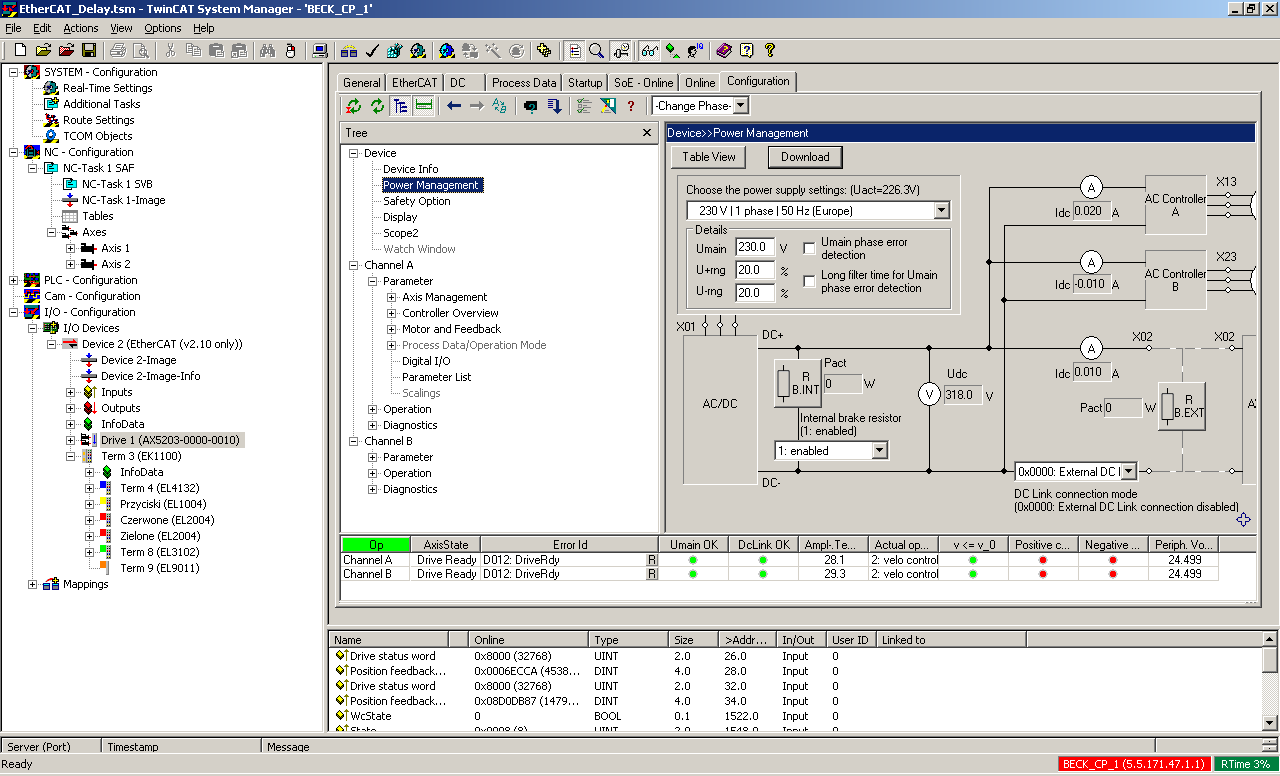
\includegraphics[width=0.9\textwidth]{images/confCP} \caption{Konfiguracja stanowiska typu CP} \label{conf:cp} \end{figure}
\begin{figure}[!htb] 	\centering 	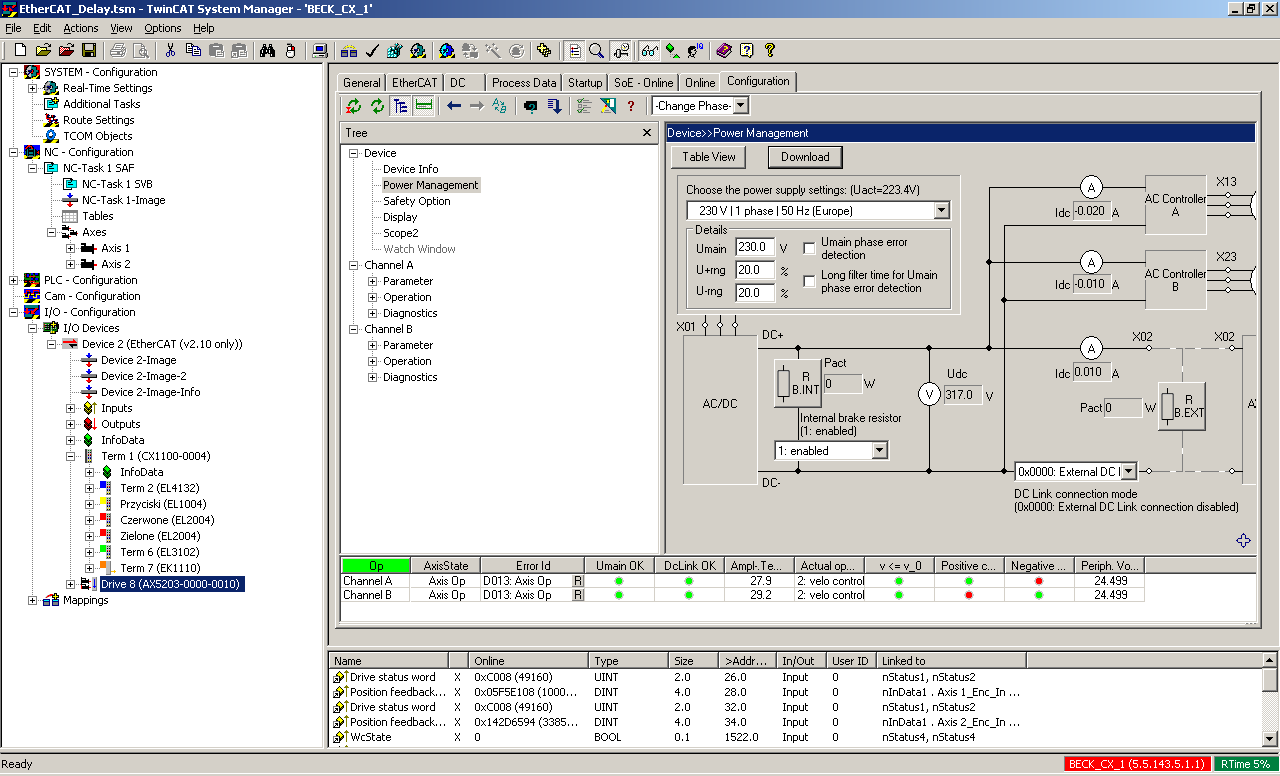
\includegraphics[width=0.9\textwidth]{images/confCX} \caption{Konfiguracja stanowiska typu CX} \label{conf:cx} \end{figure}

\subsubsection{Komputer}
Projekt w całości był realizowany na laptopie autora, podłączanym do~sieci w~laboratorium. Na~komputerze uruchomiana była maszyna wirtualna. Na~jednej zainstalowane było środowisko TwinCAT do~programowania sterownika oraz do~tworzenia i~uruchamiania wizualizacji. Wizualizacje tworzone w~środowisku TwinCAT można uruchomić bezpośrednio na~komputerze wyposażonym w~odpowiednie oprogramowanie lub na~urządzeniu docelowym po~podpięciu do~niego monitora (o~ile urządzenie docelowe posiada wyjście DVI lub odpowiedni interfejs systemowy w~postaci odrębnego modułu).

\subsection{Plan pracy}
Realizacja projektu została podzielona na następujące etapy:
\begin{itemize}
\item Zapoznanie się ze sterownikami Beckhoff oraz oprogramowaniem TwinCAT,
\item Zapoznanie się z dostępnymi serwonapędami Beckhoff,
\item Projekt i realizacja stanowiska,
\item Przygotowanie stanowiska do współpracy z systemem wizualizacji,
\item Testowanie i uruchamianie,
\item Przedstawienie projektu i~ewentualne korekty.
\end{itemize}
\indent
\indent Powyższy plan pracy stanowił dla autora wyznacznik kolejnych działań. Jednak powszechnie wiadomo, że w~praktyce poszczególne punkty są~wymienne i~wpływają na siebie wzajemnie.